\chapter{Theoretische Grundlagen}
\label{sec:grundlagen}
\pagestyle{plain}

\section{Funktionale Programmiersprachen}
\label{sec:funktionaleProgrammiersprache}
In der Programmierung gibt es zwei Programmierparadigmen, die zur Kategorisierung von Programmiersprachen dienen und sich im Laufe der Zeit entwickelt haben. %„https://de.wikipedia.org/wiki/Programmiersprache#Programmierparadigmen“)
Dabei beschreiben die Paradigmen verschiedene Prinzipien der Programmierung.
Die zugrunde liegenden Kategorien werden häufig als imperative und deklarative Programmierung bezeichnet, in welchen sich jede Programmiersprache einordnen lässt. Jede Kategorie birgt weitere Unterkategorien und dient der Verfeinerung der Prinzipien.
\begin{figure}[h]
\begin{lstlisting}[language=JavaScript]
iterative_function(n) {
  sum = 0;
  for(i = 0; i <= n; i++) {
    sum += i;
  }
}
console.log(iterative_function(10)); // => 55
\end{lstlisting}
\caption{Eine iterative Funktion}\label{fig:iterative-function}
\end{figure}
Häufig gehören funktionale Programmiersprachen dem deklarativen Programmierparadigma an. Es ist jedoch nicht ausgeschlossen, dass eine Programmiersprache mehreren Kategorien zugehörig ist und dadurch die Merkmale von mehr als einem Paradigma unterstützt. Zur Gruppe der deklarativen Programmiersprachen zählt man unter anderem Abfragesprachen wie SQL, sowie funktionale Programmiersprachen wie Lisp oder Scheme.
Programmiersprachen der deklarativen Programmierung haben ihren Ursprung in der Mathematik. Programme werden hier als mathematische Funktionen formuliert, die nicht länger beschreiben, was getan werden soll, sondern lediglich vorgeben, welches Ergebnis am Ende erwartet wird.
Bei funktionalen Programmiersprachen ist es üblich, dass eine Variable nach ihrer Initialisierung ihren zugewiesenen Wert für die gesamte Laufzeit des Programmes beibehält und unveränderlich bleibt. Es ist dementsprechend stets nachzuvollziehen, welchen Wert ein Ausdruck besitzt, wodurch insbesondere akademische Anforderungen an ein Programm, wie etwa die Beweisführung, erfüllt werden können. Zusätzlich können auch unendliche Datenstrukturen behandelt werden.
Typischerweise gibt es in funktionalen Programmiersprachen keine Schleifen, da dies bereits eine Verletzung der Unveränderlichkeit von Variablen bedeuten würde, wie klar erkennbar bei der Iteration in Abbildung~\ref{fig:iterative-function} ist. Hier wird bei jedem Durchlauf der Schleife die Variable $i$ inkrementiert und mit dem neuen Wert versehen. Es ist allerdings auch möglich eine Schleife in einer funktionalen Programmiersprache zu verwirklichen. In Abbildung~\ref{fig:recursive-function} ist die zuvor gezeigte iterative Funktion als rekursive Funktion implementiert worden.
\begin{figure}[hb]
\begin{lstlisting}[language=JavaScript]
recursive_function(n) {
  if (n < 1) return 0
  else return n + recursive_function(n-1);
}
console.log(recursive_function(10)); // => 55
\end{lstlisting}
\caption{Eine rekursive Funktion}\label{fig:recursive-function}
\end{figure}
In beiden Fällen ist das Ergebnis gleich, jedoch besitzt die rekursive Implementierung keinerlei Seiteneffekte. Es wird an keiner Stelle der Wert einer Variable verändert, es werden lediglich Aufrufe mit neuen Werten durchgeführt. Die iterative Implementierung verursacht hingegen zwei Seiteneffekte. Es wird sowohl die Variable $sum$, sowie $i$ bei jedem Schleifendurchlauf überschrieben. Bei der Rekursion hingegen wird  die Funktion $resursive\_function$
mit einem neuen Wert aufgerufen, ohne jemals die ursprüngliche Variable verändert zu haben.
Üblicherweise werden Funktionen in funktionalen Programmiersprachen als Funktionen höherer Ordnung angesehen. Das heißt, dass eine Funktion eine andere Funktion als Argument entgegen nehmen kann, oder eine Funktion als Rückgabewert hat. Diese Art von Funktionen ist bekannt unter dem Begriff $Lambda-Funktion$ oder $anonyme Funktion$. Eine solche Funktion hat entsprechend keinen Namen, sondern kann nur durch einen Verweis aufgerufen werden. Im folgenden Beispiel sehen wir den Aufruf einer anonymen Funktion in Elm:
\begin{equation} \label{eq:solve}
(\backslash x \rightarrow x * 2)\ [ 2, 3, 4 ] \Longrightarrow [4, 6, 8]
\end{equation}
Grundsätzlich wird mit einer solchen Lambda-Funktion ein mathematisches Abbildungsgesetz formuliert. Das mathematische Gegenstück zu Funktion~\ref{eq:solve} ist $x \rightarrow x * 2$ und beschreibt eine Funktion, die einen Eingabeparameter $x$ auf $x*2$ abbildet. Auch Elm gehört dem deklarativen Programmierparadigma an und vereinheitlicht dessen Konzepte.

\section{Grundlagen der Programmiersprache Elm}
\label{sec:Was ist Elm?}

\subsection{Geschichte}
\label{sec:Geschichte}
Elm ist eine funktionale Programmiersprache. Sie wurde im Rahmen der Bachelorarbeit „Elm: Concurrent FRP for Functional GUIs“\\
 (http://Elm-lang.org/papers/concurrent-frp.pdf)
von Evan Czaplicki entwickelt und im April 2012 offiziell veröffentlicht.
Auslöser für die Entwicklung von Elm war für Czaplicki die Schwierigkeit, ein Bild auf einer Webseite sowohl horizontal, als auch vertikal zu zentrieren. Es gab keine für ihn annehmbare, leichte Lösung für dieses Problem, ohne damit weitere Probleme zu schaffen. Unter der Leitfrage „What would web programming look like if we could restart?“ („Wie würde Web-Programmierung aussehen, wenn wir neu starten könnten?“) machte er sich Gedanken, welche Veränderungen an den aktuellen, etablierten Programmiersprachen für die Webentwicklung wünschenswert wären und entwickelte den ersten Prototypen von Elm.

\subsection{Konzept}
\label{sec:Konzept}
Elm verfolgt eine ganz eigene Implementierung des Model-View-Controller Paradigmas. Hier wird es \ac{MVU} genannt. Anhand des Beispiels in Abbildung~\ref{fig:counter} lässt sich das Muster in drei grundlegende Stationen unterteilen und erklären.
\begin{figure}[h]
	\centering  
	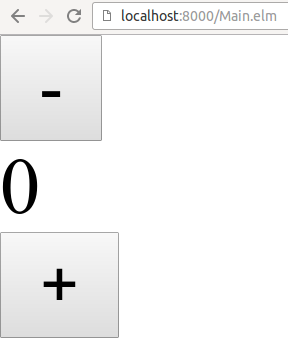
\includegraphics[scale=0.5]{img/counter.png}
	\caption{Ein simpler Zähler auf einer Webseite}\label{fig:counter}
\end{figure}
Die Abbildung~\ref{fig:counter} zeigt einen simplen Zähler der über zwei Knöpfe inkrementiert und dekrementiert werden kann. Der aktuelle Stand des Zählers wird zwischen den Knöpfen angezeigt und kann sowohl negative, als auch positive Werte annehmen.
Der angezeigte Zählerwert ist das sogenannte $Model$ und zeigt den aktuellen Status der Applikation an. Interagiert ein Nutzer nun mit einem der beiden Knöpfe um den Zähler zu erhöhen oder zu reduzieren, wird diese Aktion an die sogenannte $Update$-Funktion weitergegeben. Zusätzlich zur auszuführenden $Aktion$, bekommt diese Funktion auch noch das aktuelle $Model$, sprich den momentanen Zählerwert übergeben.
Die $Update$-Funktion nimmt sämtliche Einwirkungen durch den Nutzer von außen entgegen und wendet diese Aktionen auf das aktuelle $Model$ an. Das bedeutet in diesem konkreten Fall, dass das $Model$ erhöht oder reduziert wird. Dabei wird jedoch nicht das $Model$ direkt verändert, sondern ein neues $Model$ mit den geänderten Werten wird zurückgegeben, da sonst ein Seiteneffekt die Folge wäre. Damit dieser Vorgang zügig vonstatten geht, nutzt Elm persistente Datenstrukturen, womit nur die tatsächlich geänderten Attribute eines Models im neuen $Model$ gesetzt werden, die unveränderten Attribute hingegen werden übernommen.
Das Ergebnis der Update-Funktion wird weitergereicht an die $View$-Funktion. Sie beschreibt das Aussehen der Website, soll heißen wie das $Model$ dargestellt wird. Elm nutzt ein virtuelles \ac{DOM}, wodurch nur tatsächliche Änderungen im Browser angezeigt werden, anstatt dauerhaft das komplette \ac{DOM} stetig zu aktualisieren. Das \ac{DOM} beschreibt die Schnittstelle zum Datenzugriff auf das Objektmodell eines \ac{HTML}-Dokumentes.
Der Datenfluss in Elm wird noch einmal in Abbildung~\ref{fig:elm-model-view-update-concept} visualisiert.
\begin{figure}[h]
  \centering  
  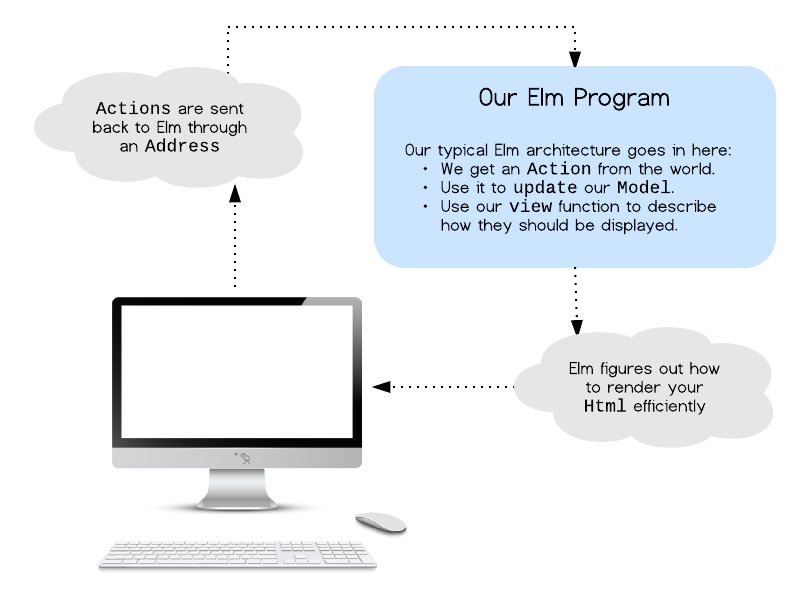
\includegraphics[scale=1]{img/elm-model-view-update-concept.png}
  \caption{Das Model-View-Update Konzept von Elm}\label{fig:elm-model-view-update-concept}
\end{figure}

\subsection{Umsetzung}
\label{sec:Umsetzung}
Der vom Programmierer verfasste Programmcode wird vor der endgültigen Nutzung zu \ac{JS}, \ac{HTML} und \ac{CSS} kompiliert und in die Webseiten integriert. Entsprechend fungiert in Elm verfasster Code im Endeffekt wie natives \ac{JS}, nutzt allerdings noch einige weitere vertiefende Konzepte, um viele Problematiken von \ac{JS} zu umgehen und auszumerzen.
Unter anderem verspricht Elm, dass generierter Code keinerlei Laufzeitfehler (http://elm-lang.org/) erzeugt. Sämtliche Fehlerquellen werden vom Compiler zuvor erkannt, abgefangen und an den Programmierer weitergeleitet, um sie zu beheben. Damit dies funktioniert, implementiert Elm mehrere Konzepte des deklarativen Programmierparadigmas.

\subsubsection{Keine Seiteneffekte}
\label{sec:Keine Seiteneffekte}
Ein Seiteneffekt beschreibt die mehrmalige Zuweisung einer Variable mit einem Wert. In Elm ist das allerdings nicht möglich. Sämtliche Variablen sind unveränderlich und können nur einmalig mit einem Wert initiiert werden. Danach bleibt diese Variable bis zum Ende der Laufzeit unverändert. Wie bereits beschrieben gibt es in Elm das Model, welches die Informationen über den Status der Applikation darstellt. Beschreibt das $Model$ beispielsweise den aktuellen Stand eines Zählers und wird dieser erhöht, muss auch das Model, um aktuell zu bleiben, verändert werden. Hier käme es zu einem Seiteneffekt. Realisiert wird diese Veränderung dadurch, dass ein neues Model mit den gleichbleibenden Daten, sowie dem zu ändernden, aktualisierten Wert erstellt wird. Da ein neues Model erstellt wurde, gibt es nun keinen Seiteneffekt mehr. Das vorherige $Model$ wird schlichtweg verworfen und mit einem neuen Model ersetzt.
Das Konzept der unveränderbaren Werte wurde aus der Mathematik übernommen.  Um Funktionen und ihre Korrektheit garantieren zu können, wird dort dasselbe Prinzip der unveränderlichen Variablen angewandt. Betrachtet man beispielsweise den Ausdruck~\ref{eq:imperative_equation}, so fällt auf, dass die Schreibweise lediglich in den meisten imperativen Programmiersprachen sinnvoll ist, allerdings einen Seiteneffekt darstellt.
\begin{equation} \label{eq:imperative_equation}
x = x + 1
\end{equation}
In einer imperativen Programmiersprache wird der Ausdruck~\ref{eq:imperative_equation} den aktuellen Wert in $x$ auslesen, um $1$ inkrementieren und das Ergebnis der Operation in die Variable $x$ schreiben.
Mathematisch betrachtet ist diese Aussage jedoch schlichtweg falsch, denn es existiert kein $x$, welches diese Aussage wahr werden lässt:
\begin{equation} \label{eq:mathematical_equation}
x=x+1 \leftrightarrow 0=1
\end{equation}
Die meisten imperativen Programmiersprachen nutzen das rechtsassoziative Gleichheitszeichen als Zuweisung, während es in der Mathematik als Vergleichsoperator angesehen wird.
Die eigentliche Bedeutung des Ausdrucks~\ref{eq:imperative_equation} ist mathematisch ausgedrückt:
\begin{equation} \label{eq:true_equation}
x_1:= x_0 + 1
\end{equation}
Es ist klar erkennbar, dass $x_1$ und $x_0$ nicht dieselbe Variable sind wodurch die Aussage nun als wahr eingestuft werden kann. Das beschriebene Konzept wird referentielle Transparenz genannt und beschreibt die Kontinuität des Wertes einer Variable.
Des Weiteren basieren Funktionen in Elm auf dem Konzept von reinen Funktionen($pure\,functions$). Das bedeutet, dass eine Funktion stets das gleiche Ergebnisse liefert, insofern auch die Eingabeparameter gleich bleiben, unabhängig vom Zeitpunkt der Ausführung. Beispiele für eine reine Funktion sind $sin(x)$ oder $add(x, y)$. Sie berechnen immer dieselben Werte, völlig unabhängig davon, wie oft oder zu welchem Zeitpunkt sie ausgeführt werden. Ein beliebtes Gegenspiel ist die $random()$ Funktion, die einen (semi-)zufälligen Wert zurückliefert und somit als eine unreine Funktion gilt. Doch auch diese Funktion kann zu einer reinen Funktion gemacht werden, wenn man sie einen Wert abhängig von einem Übergabeparameter berechnen lässt wie beispielsweise $random(seed)$.

\subsubsection{Elm-Compiler}
\label{sec:Elm-Compiler}
Laufzeitfehler sollen mit Elm in Vergessenheit geraten. Dafür soll der integrierte Compiler sorgen. Die Fehlermeldungen des Compilers sind sehr strikt und deuten exakt auf die Programmzeile die für den jeweiligen Fehler verantwortlich ist. Bei der herkömmlichen Entwicklung eines Frontends mit \ac{JS} trifft man häufig auf den Wert $undefined$. Dieser Wert beschreibt, dass die dazugehörige Variable noch nicht initialisiert wurde und somit keine nutzbaren Daten enthält. Trifft man nun auf diesen Wert und versucht eine andere Funktion darauf auszuführen, so kann das geschriebene Programm entsprechend abstürzen. Der Elm Compiler überprüft den Programmcode nach exakt diesen Situation beziehungsweise analysiert, ob Variablen und Funktionen vorab initialisiert wurden, welche Parameter die einzelnen Funktionen erwarten und ob die Rückgabeparameter dem Typen entsprechen, den die anderen Funktionen erwarten. Befolgt man die Anweisungen des Compilers, soll das in einem stark strukturierten, lesbaren und funktionieren Code münden.
Dem Programmierer werden weniger Möglichkeiten gegeben, bestimmte Ziele zu erreichen, doch dadurch soll auf lange Sicht einheitlicher, lesbarer und besser zu wartender Code erzeugt werden. Passend dazu gibt es bereits viele Erweiterungen für gängige Editoren wie Sublime Text und Atom, welche beim Speichern des Projektes den Code entsprechend des Style Guides strukturieren und formatieren. So kann einerseits die Lesbarkeit des Codes vereinheitlicht, andererseits die Fehlerquellen in Form von Einrückungsfehlern oder vergessenen Kommas o.ä. verringert werden.

\subsubsection{Statische Typisierung}
\label{sec:Statische Typisierung}
Anders als bei nativem \ac{JS}, gibt es in Elm keine dynamische Typisierung. Das bedeutet, dass sowohl die Typen einer Variable, als auch die Rückgabewerte von Funktionen bereits bei der Kompilierung bekannt sein müssen. Natives \ac{JS} erlaubt es, dass die Typen von Variablen erst zur Laufzeit überprüft werden und sich zusätzlich in dieser Zeit ändern können. So ist der Quellcode in Abbildung~\ref{fig:dynamische-typisierung} konform in \ac{JS}.
\begin{figure}[ht]
\begin{lstlisting}[language=JavaScript]
var i = 1;
i = "Test";
\end{lstlisting}
\caption{Beispiel der dynamischen Typisierung}\label{fig:dynamische-typisierung}
\end{figure}
Der Typ der Variable $i$ wurde in der Abbildung~\ref{fig:dynamische-typisierung} während der Laufzeit von $number$ zu $string$ geändert. Da Elm stark typisiert ist, gibt es keine Möglichkeit, dass eine Funktion verschiedene Datentypen zurück gibt oder eine Variable mehrere Typen während der Laufzeit annimmt.

\subsubsection{Modularität}
\label{sec:Modularität}
Um geschriebenen Code auch in Zukunft wartbarer zu machen, ist Elm modular aufgebaut und leicht erweiterbar. Es ist denkbar einfach vorhandenen Code zu importieren. Die importierten Module verstehen sich als gekapselt, wodurch sie in keiner Weise mit dem bereits verfügbaren Code kollidieren können.


\subsubsection{Performanz}
\label{sec:Performanz}
\begin{figure}[hb]
  \centering  
  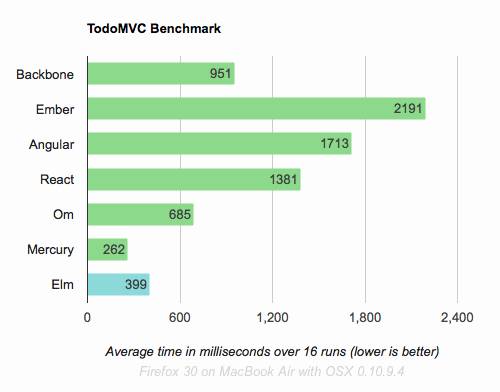
\includegraphics[scale=0.6]{img/virtual-dom.png}
  \caption{Performanz von Elm im Vergleich zu anderen Web-Frameworks. \cite{elm-performance}}\label{fig:performance}
\end{figure}
Obwohl Daten nicht verändert, sondern lediglich als neuer aktualisierter Datensatz betrachtet werden und einzelne Funktionen stark ausgelagert werden können, leidet die Performanz nicht darunter. Laut Abbildung~\ref{fig:performance} überzeugt Elm mit einer sehr guten Geschwindigkeit. Möglich wird das durch die Verwendung eines virtuellen \ac{DOM}.
Dabei wird das echte \ac{DOM} bei jedem „Frame“ in eine abstrakte Version kopiert. Auf diese abstrakte Version werden die Änderungen angewandt. Zunächst klingt diese Vorgehensweise sehr langsam und aufwändig, doch um die Geschwindigkeit zu gewährleisten wird das aktuelle abstrakte \ac{DOM} mit dem neuen, veränderten \ac{DOM} verglichen und nach Unterschieden gesucht. Jede Unterschiedlichkeit wird daraufhin zu einer Liste hinzugefügt, in der sämtliche Änderungen festgehalten werden. Anschließend wird diese Liste an den Browser zurückgegeben, so dass alle Änderungen für den Nutzer sichtbar gemacht werden können. Daraus resultiert, dass nur noch die tatsächlich neuen Elemente im \ac{DOM} des Nutzers aktualisiert werden müssen. Dieser zu verändernde Teil stellt nur einen Bruchteil des kompletten \ac{DOM} dar. Man kann dadurch von einer immensen Effizienzsteigerung ausgehen.


\subsubsection{Interoperabilität}
\label{sec:Interoperabilität}
Es wäre sehr aufwendig die gängigsten JavaScript-Bibliotheken und -Frameworks wie jQuery oder AngularJS komplett zu verwerfen und mit Elm zu realisieren respektive neu zu programmieren. Glücklicherweise bietet Elm eine ausgereifte Interoperabilität, wodurch alle Garantien der deklarativen Programmierung übernommen werden können, selbst wenn die externen Bibliotheken diese nicht gewährleisten.
Die genannten externen Bibliotheken sind zum Großteil nicht deklarativ programmiert, weswegen normalerweise keinerlei Garantien seitens Elm gemacht werden können. Jedoch ist Elm von den externen Bibliotheken isoliert und kommuniziert nur über sogenannte Ports mit JavaScript. Die Kommunikation durch die Ports funktioniert in beide Richtungen, womit sämtliche Daten bei Bedarf ausgetauscht werden können. Da in Elm wie bekannt vorab die Typen der Eingabeparameter und Rückgabewerte spezifiziert werden müssen, werden die Garantien weiterhin gewahrt.

\subsubsection{Debugger}
\label{sec:Debugger}
Nicht nur die detaillierten Fehlermeldungen des Compilers sind ein großer Pluspunkt von Elm, sondern auch der mitgelieferte und einfach zu bedienende Debugger. Anders als bei anderen Programmiersprachen zeigt der Debugger nicht nur einen einfachen Stacktrace mit den letzten Rücksprungadressen an. Vielmehr ermöglicht es der Debugger in Elm die Zeit zurückzudrehen. In gängigen Debuggern ist es nicht einfach, ein bestimmtes Verhalten, das möglicherweise zum Absturz des Programms geführt hat, zu reproduzieren. Um den Fehler erneut zu erhalten und dadurch ein Verständnis des Fehlers aufzubauen ist es oft notwendig den genauen Hergang und Ablauf manuell nachzuahmen. Der Elm Debugger hingegen speichert den Status einer jeden Variable zu jedem Zeitpunkt und zeichnet außerdem die Wechsel auf. Aufgrund dessen ist es sehr einfach möglich mit Hilfe eines Sliders auf der Website die Zeit buchstäblich zurückzudrehen und den vorherigen Status wieder aufzurufen. Weiterhin besteht die Möglichkeit sämtliche Daten zu diesem Zeitpunkt zu betrachten und live zu verändern. Dadurch wird nicht nur der aktuell begutachtete Status verändert und der Effekt zeitgleich auf dem Bildschirm angezeigt, sondern auch alle folgenden Status mitsamt den Daten werden entsprechend aktualisiert. Evan Czaplicki hat dahingehend ein Video angefertigt, dass den Vorgang sehr detailliert beschreibt (LINK). Alternativ kann die Abbildung XY betrachtet werden, die einen Zeitstrahl mit Werten, sowie die Möglichkeiten die sich durch den Debugger ergeben, aufzeigt.


\subsubsection{Praktische Anwendungsgebiete}
\label{sec:Praktische Anwendungsgebiete}
Elm ist noch recht neu und befindet sich im ständigen Wandel. Für viele Entwickler ist Elm entsprechend noch keine wirkliche Alternative zu ihren gegenwärtig genutzten Frameworks, obgleich die Entwicklung mit den gängigen Werkzeugen oftmals steinig ist. Nur wenige Unternehmen nutzen derzeit Elm in ihrem Produktionsumfeld. Die wohl derzeit größten Nutzer sind NoRedInk, Prezi und CircuitHub. Alle Betriebe überführen Stück für Stück bereits bestehende Teile ihres Frontends zu Elm. NoRedInk gibt an, dass der überführte Elm-Code in den letzten acht Monaten keinerlei Laufzeitfehler erzeugt hat, anders als die vorherige Implementierung\\ (https://www.youtube.com/watch?v=zBHB9i8e3Kc). Dennoch wird es wohl noch eine Weile dauern, bis sich mehr Firmen der Vorstellung hingeben ihr lauffähiges System in die vielversprechende Programmiersprache Elm zu portieren, nicht zuletzt, weil sie sich noch in einem sehr frühen Stadium befindet und somit noch nicht völlig ausgereift ist.
Es existiert jedoch bereits eine Vielzahl an Projekten die mit Elm verwirklicht wurden. Dabei sind viele dieser Projekte kleinere Retro-Spiele, die über den Browser gespielt werden können \footnote{\cite[vgl.]{builtwithelm}}. Dazu gehört unter anderem Tetris, Pong und Space Invaders. Weiterhin bietet Elm sehr einfache Möglichkeiten Formen wie Kreise, Vierecke, Hexagone und vieles mehr zu erzeugen, ohne großartig in die Mathematik einzusteigen.\\
Dieser Einblick zeigt bereits, dass Elm in vielerlei Hinsicht Besserung für die Entwicklung von Webapplikationen verspricht. Doch wie praktikabel sind diese Versprechungen? Ist die Programmiersprache effizient und intuitiv, oder durch ihr noch frühes Entwicklungsstadium unausgereift?
„The best functional programming in your browser“ - Diese Aussage wird anhand verschiedener Bewertungskriterien überprüft.
Im Zuge dessen wird eine Webseite mit kleineren Modulen in Elm erzeugt. Die fertige Webseite respektive der erzeugte Quellcode wird anhand der zuvor erstellten Bewertungskriterien ausgewertet. Auch die Beobachtungen während der Entwicklung, wie etwa unvorhergesehene Probleme, gehen mit in die Wertung ein.

\subsection{Einführung in die Elm-Architektur}
\label{sec:elm-architektur}
TODO: Evtl. Absatz \nameref{sec:Praktische Anwendungsgebiete} hier rein mergen und abändern?
... Um eine Programmiersprache jedoch anzuwenden, ist es notwendig zuvor die Architektur kennenzulernen. Dieses Kapitel soll eine Einführung in die Programmiersprache Elm darstellen und die grundlegenden Funktionen näher bringen.

\subsubsection{Elm-REPL}
\label{sec:elm-repl}
Ein nützliches Tool um mit Werten in Elm zu interagieren und kleinere Algorithmen zu testen, ist die $elm-repl$. \ac{REPL} bezeichnet dabei die Iteration, welche ein Algorithmus durchlebt. Zunächst wird der Quellcode gelesen (read), danach ausgewertet (evaluate) und das Ergebnis ausgegeben (print). Dieser Vorgang wiederholt sich (loop), bis die Entwicklung fertig ist. $Elm-repl$ wird über die Kommandozeile aufgerufen und gestartet. In Abbildung~\ref{fig:elm-repl} ist das Tool abgebildet und zeigt beispielhafte Eingaben und Evaluierungen.
\begin{figure}[h]
\centering
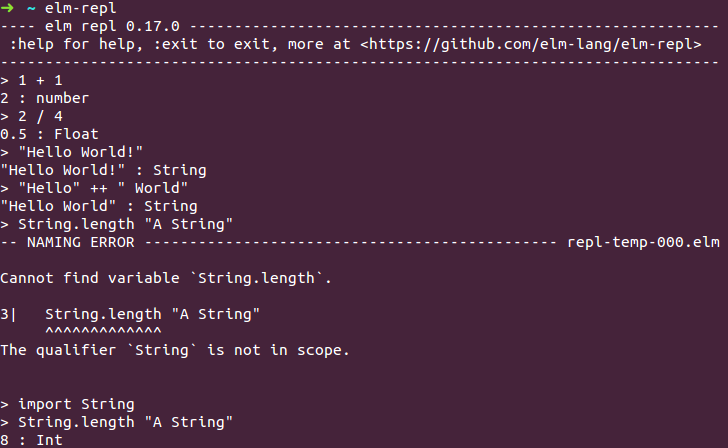
\includegraphics[scale=0.5]{img/elm-repl.png}
\caption{Das Tool elm-repl in der Kommandozeile}\label{fig:elm-repl}
\end{figure}
Wie aus der Abbildung~\ref{fig:elm-repl} ersichtlich wird, werden auch Fehler ausgegeben. In diesem Beispiel wurde versucht auf die Bibliothek $String$, genauer die Funktion $length$ zuzugreifen. Diese Bibliothek wurde allerdings noch nicht eingebunden, wodurch es zu dem Fehler kam. Nachdem die Bibliothek über das Kommando $import String$ importiert wurde, war der Fehler behoben. Die $elm-repl$ erlaubt es, alle Bibliotheken die das Paket $core$ mitliefert, zu importieren.

\subsubsection{Basisdatentypen}
\label{sec:Basisdatentypen}
Elm hat nur eine geringe Anzahl an Basisdatentypen, mithilfe derer sämtliche weiterführende Konstrukte abgeleitet werden können:
\begin{itemize}
	\item 42 : number
	\item True : Bool
	\item 'a' : Char
	\item {[1, 2, 3] : List}
\end{itemize}
Durch die Kombination dieser Basisdatentypen können weitere komplexere Datentypen wie $Strings$, $Integer$ oder $Floats$, wie es in Abbildung~\ref{fig:elm-repl} zu sehen ist, erzeugt werden.

\subsubsection{Basisfunktionen}
\label{sec:Basisfunktionen}
Elm kommt mit einer Vielzahl an grundlegenden Funktionen, um notwendige arithmetische Operationen zu ermöglichen. Dazu gehören Funktionen zur Addition ($+$), Subtraktion ($-$), Multiplikation ($*$) und Division ($/$). Um Vergleiche zu vollziehen gibt es die Funktionen zur Prüfung der Gleichheit ($==$) und Ungleichheit($/=$). Wie in Abbildung~\ref{fig:elm-repl} zu sehen ist, können zwei $String$s zu einem verbunden werden, indem die Funktion $++$ angewendet wird.

\subsubsection{Union Types}
\label{sec:Union-Types}
In vielen Applikationen können Datentypen unterschiedliche Zustände annehmen. So kann beispielsweise ein $Tag$ die Zustände $Montag$ bis $Sonntag$ annehmen. Die in anderen Programmiersprachen als $algebraische Datentyp$ bekannte Aufzählung von Zuständen wird in Elm $Union\,Type$ genannt und beschreibt auch hier eine Aufzählung von endlich vielen Zuständen eines Datentypen. Die Einführung eines solchen $Union\,Type$s erlaubt es dem Compiler den Quellcode auf fehlende Zustände zu überprüfen. Ist es zum Beispiel das Ziel, eine Meldung abhängig vom aktuellen Wochentag auszugeben, müssen alle Zustände und ihre Folge dafür deklariert werden. Fehlt eine Deklaration, kann der $Elm-Compiler$ dies anhand des $Union\,Type$s erkennen.
\begin{figure}[h]
\begin{lstlisting}[language=Elm]
type Day = Monday | Tuesday | .. | Sunday
storeStatus : Day -> String
storeStatus day =
  case day of
    Monday ->
      "Opened"
    Sunday ->
      "Closed"
\end{lstlisting}
\caption{Ein Union-Type in Elm}\label{fig:elm-union-type}
\end{figure}
Betrachtet man die Abbildung~\ref{fig:elm-union-type} ist klar erkennbar, dass die Funktion $storeStatus$ nicht alle Fälle, die der Typ $Day$ annehmen kann, behandelt werden. Aufgrund der vorherigen Deklaration eines $Union\,Type$ kann der $Elm-Compiler$ einsehen, welche möglichen Zustände der Typ $Day$ annehmen kann. Dadurch wird ein Fehler geworfen, insofern die fehlenden Typen nicht ergänzt werden. Dieses Konzept der algebraischen Datentypen erscheint zunächst sehr ähnlich den $Enumerationen$ in beispielsweise $C++$ oder anderen Programmiersprachen. Tatsächlich gibt es diese Form der Datenabstraktion in einer Vielzahl von funktionalen Programmiersprachen, mit dem wohl bekanntesten Vertreter der funktionalen Programmiersprache $Haskell$. Der Vorteil eines $Union\,Type$s in Elm gegenüber $Enumerationen$ in C++ oder Java ist, dass jeder Zustand der Aufzählung optionale Parameter übergeben bekommen kann. Damit bietet sich die Möglichkeit viel detailliertere Konstrukte zu erzeugen, ohne die Typensicherheit die sich durch die $Union\,Type$s ergibt zu verlieren. Das Beispiel der Abbildung~\ref{fig:elm-union-type} könnte entsprechend erweitert werden, so dass die Tage $Montag$ bis $Freitag$ zusätzlich noch eine Öffnungszeit besitzen.
\begin{figure}[h]
\begin{lstlisting}[language=Elm]
type Day = Monday Int Int | .. | Sunday
storeStatus : Day -> String
storeStatus day =
  case day of
    Monday start end->
      "Opened from:"
      	++ start "until"
      	++ end
    Sunday ->
      "Closed"
\end{lstlisting}
\caption{Ein erweiterter Union-Type in Elm}\label{fig:elm-union-type-advanced}
\end{figure}
Wie in Abbildung~\ref{fig:elm-union-type-advanced} zu sehen ist, wurden die einzelnen Tage in der Deklaration um die Parameter $Int$ erweitert. In diesem Fall sollen die $Integer$ vereinfacht die Start- und Endzeit der Öffnungszeit widerspiegeln. Auffällig ist, dass die Signatur der Funktion $storeStatus$ im Vergleich zur vorherigen Abbildung~\ref{fig:elm-union-type} nicht verändert wurde. Der übergebene Datentyp ist noch immer ein $Day$, mit dem Zusatz, dass die Wochentage zwei weitere Parameter $start$ und $end$ besitzen. Auf diese Weise können komplexe Konstrukte definiert werden, während die Typensicherheit gewährt bleibt.

\subsubsection{Records}
\label{sec:Records}
Eine weitere Datenstruktur in Elm sind die sogenannten $Records$. Ein $Record$ ist vergleichbar mit einem $Objekt$ in \ac{JS} und verfolgt eine sehr ähnliche Syntax. Es ist möglich, eigene Felder in einem $Record$ zu definieren, mit allen Datentypen die bisher erzeugt wurden. Dazu gehören nicht nur die Basis-Datentypen, sondern auch alle daraus konstruierten. Auch können verschiedene Datentypen in einem $Record$ kombiniert werden.
\begin{figure}[h]
\begin{lstlisting}[language=Elm]
university = { typ = "Fachhochschule"
             , gruendungsdatum = 1969
             , ort = "Kiel" }
university.typ  --> "Fachhochschule"
.ort university --> "Kiel"

{university | ort = "Flensburg" }
\end{lstlisting}
\caption{Ein Record in Elm}\label{fig:elm-record}
\end{figure}
In Zeile $1$ der Abbildung~\ref{fig:elm-record} ist erkennbar, wie ein $Record$ mit initialen Werten erstellt wird. Lediglich das Gleichheitszeichen für die Zuweisung unterscheidet sich hierbei von herkömmlichen erstellen eines $Records$ in \ac{JS}. Um ein Feld in einem $Record$ direkt anzusprechen, kann die übliche Schreibweise aus Zeile $4$ gewählt werden. Zeile $5$ hingegen führt zum gleichen Ergebnis, nutzt intern jedoch eine $anonyme\,Funktion$. Der Unterschied eines $Records$ im Gegensatz zu einem $Objekt$ in \ac{JS} liegt darin, dass Felder nicht dynamisch hinzugefügt oder gelöscht werden können. Sobald ein Feld definiert wurde, ist es für die gesamte Laufzeit vorhanden. Die einzige Möglichkeit einen $Record$ zu verändern liegt darin, den Inhalt der Felder zu manipulieren. Zeile $7$ der Abbildung~\ref{fig:elm-record} zeigt, wie das Feld $Ort$ des $Records$ mit einem neuen Wert versehen wird. Dabei ist zu beachten, dass aufgrund der Unveränderlichkeit einer Datenstruktur in Elm nicht der $Record$ selbst verändert wird. Viel mehr wird ein neuer $Record$ erstellt, der die Änderung, sowie gleichbleibenden Felder des alten $Record$ annimmt. Ein weiterer Unterschied gegenüber \ac{JS} ist, dass ein Feld nie den Wert $undefined$ oder $null$ annehmen kann, da eingeführte Felder stets initialisiert werden müssen. Des Weiteren ist es nicht möglich rekursive Felder zu erzeugen.

\subsubsection{Tupel}
\label{sec:Tupel}
Sollte es notwendig sein, mehr als einen Wert als Rückgabewert zu haben, so bietet sich die Nutzung von $Tupel$n an. Ein $Tupel$ ist eine weitere Datenstruktur in Elm und kann eine beliebig feste Anzahl an Werten beinhalten. Jeder Wert ist unabhängig von den anderen und kann einen geeigneten Datentyp annehmen. Die folgende Abbildung~\ref{fig:elm-tupel} zeigt, wie ein solches Tupel von einer Funktion zurückgegeben werden kann.
\begin{figure}[h]
\begin{lstlisting}[language=Elm]
type Food = { name: String, sort: String }

isCookie : Food -> (Bool, String)
isCookie food =
  if food.sort == "cookie" then
    (True, food.name)
  else
    (False, "No cookie.")

isCookie { name = "Oreo", sort = "cookie" }
--> (True, "Oreo")
\end{lstlisting}
\caption{Ein Tupel in Elm}\label{fig:elm-tupel}
\end{figure}
Der Rückgabewert des beispielhaften Aufrufes in Zeile $10$ ist ein Tupel, bestehend aus einem $Bool$ und einem $String$, wie es in der Signatur in Zeile $3$ definiert wurde. Soll das Tupel noch weiter verwendet werden, liefert die Bibliothek $Basics$ aus dem Paket $elm-lang/core$ die Funktionen $fst$ und $snd$, die entsprechend den ersten oder zweiten Wert eines Tupels zurückliefern. Auf diese Weise kann ein einzelner Wert des Tupels extrahiert werden. Aufgrund der fehlenden Wege Tupel mit mehr als zwei Werten auszuwerten, sollte nur bedingt auf Tupel zurückgegriffen und stattdessen ein $Record$ verwendet werden.

\subsubsection{Variablen}
\label{sec:Variablen}
Die Lebenszeit eines $Records$ ist die gesamte Laufzeit des Programmes. Eine $Variable$ in Elm hingegen bleibt nur für die Dauer der Funktion in der sie definiert wurde erhalten und ist auch nur in diesem Namensraum gültig. Außerhalb der Funktion ist die Variable nicht mehr bekannt. In Elm wird eine Variable innerhalb eines $let..in$-Konstrukts erzeugt. $Let$ bezeichnet dabei den Abschnitt, in welchem sämtliche Variablen erstellt werden und einen Wert zugewiesen bekommen. Die innerhalb dieses Blockes definierten Variablen können dabei aufeinander zugreifen, unabhängig von ihrer Reihenfolge. Mit Hilfe des $let..in$-Blockes kann die Logik einer Funktion noch weiter ausgelagert werden, ohne eine explizit neue Funktion zu definieren.
\begin{figure}[h]
\begin{lstlisting}[language=Elm]
meaningOfLife =
  let
    fourtyTwo = oneHundred - 58
    oneHundred = 100
  in
    fourtyTwo

meaningOfLife --> 42
\end{lstlisting}
\caption{Eine Variablendeklaration in Elm}\label{fig:elm-variables}
\end{figure}
Abbildung~\ref{fig:elm-variables} zeigt beispielhaft die Deklaration einer Funktion $meaningOfLife$, die innerhalb des $let..in$-Blockes die Variablen $fourtyTwo$ und $oneHundred$ deklariert und ihnen einen Wert zuweist. Die Inhalte eines $let..in$-Blockes müssen eingerückt werden, während hingegen eine übliche Funktion auch in einer Zeile verfasst werden kann. Des Weiteren ist erkennbar, dass die Variable $oneHundred$ erst nach der Deklaration von $fourtyTwo$ deklariert wird, jedoch bereits vorher nutzbar ist. Der $elm-compiler$ optimiert diese Programmstelle während des Kompiliervorganges entsprechend. Die beiden deklarierten Variablen sind lediglich in dem definierten $let..in$-Block verfügbar. Eine Verwendung außerhalb des Blockes hätte einen Compilerfehler zur Folge. Es besteht ferne die Möglichkeit ganze Funktionen innerhalb des Blockes zu definieren und zu nutzen.

\subsubsection{Kontrollstrukturen}
\label{sec:Kontrollstrukturen}
Elm bietet die Möglichkeit verschiedene Kontrollstrukturen anzuwenden. Dabei wird ein Record auf mögliche Werte hin überprüft und abhängig vom Wert ein anderer logischer Pfad gewählt.
\begin{figure}[h]
\begin{lstlisting}[language=Elm]
isItACookie food =
  if food == "cookie" then
  	True
  else if food == "grapefruit" then
    False
  else
    False
\end{lstlisting}
\caption{Eine Konstrollstruktur in Elm}\label{fig:elm-conditional}
\end{figure}
In Abbildung~\ref{fig:elm-conditional} ist eine herkömmliche $if$-Abfrage zu sehen. In Elm sind die Schlüsselwörter $if$, $then$ und $else$ notwendig und unterteilen die Bedingung von der angewandten Folge, die nach dem Schlüsselwort $then$ folgt. Insofern keine $if$-Bedingung zutrifft, wird der $else$-Fall angewandt.
Elm verfolgt auch hier die statische Typisierung und fordert, dass jede mögliche Verzweigung denselben Typen zurückliefert. Eine Bedingung muss in Elm immer $True$ oder $False$ liefern und somit einen $Bool$ liefern. In anderen Programmiersprachen wie beispielsweise $C++$ evaluiert eine Bedingung zu $True$, wenn sie nicht $0$ oder $false$ ist. Am Beispiel in Abbildung~\ref{fig:cpp-conditional} sieht man, dass $0$ zu $false$ auswertet. In Elm hingegen meldet der $elm-compiler$ einen Fehler, sobald eine Bedingung zu einem anderen Typen als $Bool$ auswertet.
Abbildung~\ref{fig:elm-union-type} zeigt, wie $Union\,Type$s überprüft werden können. Die Kontrollstruktur ähnelt dabei dem $switch$-$case$-Konstrukt von anderen Programmiersprachen wie \ac{JS} oder C++.
\begin{figure}[h]
\begin{lstlisting}[language=cpp]
string whatIsZero() {
  if (0) return "0 equals to TRUE";
  else return "0 equals to FALSE";
}
cout << whatIsZero() << endl;
//=> 0 equals to FALSE

\end{lstlisting}
\caption{Konstrollstruktur in C++}\label{fig:cpp-conditional}
\end{figure}

\subsubsection{Funktionen}
\label{sec:Funktionen}
Um in irgendeiner Art und Weise eine Interaktion mit den erstellten $Records$ zu vollziehen, benötigt der Entwickler auch in Elm eine Funktionen. Solch ein Programmkonstrukt wird mittels eines Funktionsnamen und dem Gleichheitszeichen realisiert.
\begin{figure}[h]
\begin{lstlisting}[language=Elm]
add : Int -> Int -> Int
add a b =
  a + b

add 3 4  --> 7
\end{lstlisting}
\caption{Eine Funktion in Elm}\label{fig:elm-function}
\end{figure}
Abbildung~\ref{fig:elm-function} zeigt, wie eine simple Addition zweier Integer-Werte umgesetzt wird. Die Buchstaben $a$ und $b$ deuten an, dass die Funktion $add$ zwei Parameter erwartet. Der gesamte Inhalt nach dem Gleichheitszeichen ist der sogenannte Rumpf einer Funktion und beschreibt den anzuwendenden Algorithmus. Der Funktionsaufruf ist in Zeile 5 sichtbar. Auffällig ist, dass eine Funktion nie explizit einen Wert zurück gibt, wie es in anderen Programmiersprachen wie \ac{JS} oder C++ meist durch den Befehl $return$ geschieht. Elm gibt implizit die letzte ausführbare Zeile als Rückgabewert zurück. Der beispielhafte Aufruf der Funktion $add$ in Zeile 5 hätte dementsprechend $7$ als Ergebnis. Des Weiteren ist erkennbar, dass Elm ohne die Nutzung von Kommata oder Klammern auskommt. Klammern werden erst notwendig, wenn mehrere Funktionen geschachtelt ablaufen sollen und eine Auswertung der Befehle von links nach rechts nicht ausreicht.
Zusätzlich zu einer explizit benannten Funktion, gibt es die $anonyme$ Funktion. Sie kommt ohne einen Funktionstitel aus und wird an Funktionen höherer Ordnung weitergereicht.
$List.filter$ ist eine solche Funktion und erwartet eine anonyme Funktion als Parameter, auf Basis derer eine Liste gefiltert wird. Aus der Abbildung~\ref{fig:elm-anonym-function} wird ersichtlich, dass die übergebene Liste, bestehend aus $4$ Einträgen, auf die Präsenz des Buchstabens $a$ hin überprüft wird. Dabei wird jeweils ein Wert an die anonyme Funktion weitergereicht, die in Form der Variable $str$ repräsentiert und mit dem String $a$ auf Gleichheit überprüft wird. Einträge die diesem Vergleich entsprechen, werden einer neuen Liste hinzugefügt. Wird das Ende der zu überprüfenden Liste erreicht, wird die Ergebnisliste als Rückgabewert ausgegeben.

\subsubsection{Signaturen}
\label{sec:Signaturen}
Die jeweils erste Zeile der Abbildung~\ref{fig:elm-function} und \ref{fig:elm-anonym-function} zeigt den Aufbau einer Signatur. Solch eine Signatur beschreibt die Funktion. Dabei sind Informationen über die Anzahl und der jeweilige Typ der Übergabeparameter, sowie der Typ des Rückgabewertes enthalten. Der letzte Typ einer Signatur ist dabei immer der Rückgabewert, die vorherigen Typen stellen die Typen der Übergabeparameter in der übergebenen Reihenfolge dar. Die einzelnen Parameter sind durch einen Pfeil ($->$) voneinander getrennt. Wird eine Funktion anstelle eines einfachen Datentypen als Parameter übergeben, wird dies wie in Abbildung~\ref{fig:elm-anonym-function} durch das Einklammern der Typen angedeutet. Die Typen innerhalb der Klammer stellen wiederum die Typen der Übergabeparameter und Rückgabewerte der Funktion dar.
\begin{figure}[h]
\begin{lstlisting}[language=Elm]
List.filter : (a -> Bool) -> List a -> List a
List.filter (\str -> str == "a") ["a", "b", "c", "a"]
--> ["a", "a"]
\end{lstlisting}
\caption{Anwendung einer anonymen Funktion in Elm}\label{fig:elm-anonym-function}
\end{figure}
Anhand der Abbildung~\ref{fig:elm-function} lässt sich erkennen, dass die $add$-Funktion zwei Parameter vom Typ $Int$ erwartet und letzten Endes ein Ergebnis des Typ $Int$ liefert. Fehlt einer Funktion die Signatur, wird der $elm-compiler$ eine Warnung ausgeben und zusätzlich eine passende, jedoch teilweise allgemeinere Signatur ausgeben. Würde die Funktion in Abbildung~\ref{fig:elm-function} keine Signatur enthalten, würde der $elm-compiler$ die Signatur $add : number -> number -> number$ vorschlagen. Da ein $Int$ nur eine Spezifizierung des Basisdatentypen $number$ darstellt, ist das nicht verwunderlich. Der $elm-compiler$ nutzt implizit die eigens erarbeiteten Signaturen bei der Überprüfung des Quellcodes, sollte der Entwickler keine Signatur angegebenen haben.

\subsubsection{Typen Alias}
\label{sec:typ-alias}
Je komplexer ein Record wird, desto länger und unübersichtlicher wird auch die dazugehörige $Signatur$. Dementsprechend bietet sich eine Abkürzung der Signatur an, die in Elm als $type\,alias$ bezeichnet wird. Dabei handelt es sich um eine Repräsentation einer komplexen Datenstruktur in einer kurzen Schreibweise.
\begin{figure}[h]
\begin{lstlisting}[language=Elm]
isOldEnough : { name : String
	      , profile : String
	      , age : Int
	      } -> Bool
isOldEnough user =
	...
\end{lstlisting}
\caption{Definition einer Funktion ohne Typen Alias}\label{fig:no-type-alias}
\end{figure}
In Abbildung~\ref{fig:no-type-alias} wird eine Funktion mit einem komplexen $Record$ als Übergabeparameter beschrieben. An dieser Stelle hat der $Record$ lediglich drei Felder, führt allerdings schon zu einem recht unübersichtlichen Quellcode. Mit Hilfe des $type\,alias$ kann die Signatur gekürzt werden, indem die Repräsentation des $Records$ ausgelagert wird. In Abbildung~\ref{fig:no-type-alias} können die Auswirkung davon betrachtet werden. Nachdem der $type\,alias$ erstellt wurde, kann das Konstrukt mit dem entsprechenden $alias$ angesprochen werden. Zeile $5$ verdeutlicht, wie der $alias$ genutzt wird. Der Algorithmus der Funktion bleibt völlig unberührt, wodurch diese Änderung eher kosmetischer Natur ist.
\begin{figure}[h]
\begin{lstlisting}[language=Elm]
type alias User = { name : String
	          , profile : String
	          , age : Int
	          }
oldEnough : User -> Bool
\end{lstlisting}
\caption{Definition einer Funktion mit Typen Alias}\label{fig:type-alias}
\end{figure}

\subsubsection{Module}
\label{sec:Module}
\begin{figure}[h]
\begin{lstlisting}[language=Elm]
module MyModule exposing(..)
module MyModule exposing (add, anotherMethod)
\end{lstlisting}
\caption{Mögliche Deklarationen eines Elm-Moduls}\label{fig:elm-module}
\end{figure}
Oftmals ist es sinnvoll Quellcode der sich nur auf eine Problemlösung bezieht zu gruppieren. Auch in Elm ist es möglich Code auszulagern in sogenannte $Module$. Sie beschreiben eine Art Container, in dem der Code isoliert von den anderen Projektteilen betrachtet werden kann. Um ein $Modul$ in Elm zu erstellen, muss eine neue Datei vom Typ $elm$ erzeugt werden. Abbildung~\ref{fig:elm-module} zeigt zwei Beispiele, wie eine Quelldatei als Modul deklariert werden kann. Zeile $1$ gibt dabei sämtliche Funktionen die im Modul beinhaltet sind nach außen weiter, sobald das Modul importiert wird. Dies sollte nur gemacht werden, wenn das Modul sich um eine Art Bibliothek handelt, in der sämtliche Funktionen verfügbar gemacht werden sollen. In Zeile $2$ hingegen wird ersichtlich, wie nur ausgewählte Funktionen nach außen sichtbar gemacht werden. Auf der anderen Seite hingegen würde der Entwickler das Modul $MyModule$ importieren und daraufhin die Funktionen $add$ und $anotherMethod$ nutzen können.

\subsubsection{Importierung}
\label{sec:Importierung}
Jeder Entwickler hat ferner die Möglichkeit die zuvor erstellten Module an einer anderen Stelle zu importieren. Dabei wird das gesamte Modul in den aktuellen Namensraum geladen und nutzbar gemacht. In welcher Ausprägung die Funktionen des importierten Moduls eingebunden werden, hängt von der Spezifikation des Imports ab.
\begin{figure}[h]
\begin{lstlisting}[language=Elm]
import MyModule
import MyModule exposing(..)
import MyModule exposing (add, anotherMethod)
import MyModule as MyVeryOwnModuleName
\end{lstlisting}
\caption{Mögliche Formen der Importierung eines Elm-Moduls}\label{fig:elm-import-module}
\end{figure}
Die Abbildung~\ref{fig:elm-import-module} zeigt vier mögliche Arten das Modul $MyModule$ zu importieren. Zunächst einmal werden alle Funktionen, die das Modul selbst über das Stichwort $exposing$ freigibt geladen. Das Einbinden wie in Zeile $1$ hat zur Folge, dass sämtliche Funktionen mit dem expliziten Modulnamen voran angesprochen werden müssen. Die Funktion $add$ wird beispielsweise mit $MyModule.add$ aufgerufen. Zeile $2$ wiederum hat zur Folge, dass alle Funktionen des Moduls $MyModule$, darunter auch die Funktion $add$, in den Namensraum des aktuellen Moduls geladen werden. Logischerweise ist an dieser Stelle für den Aufruf der $add$-Funktion nichts weiter notwendig, außer wenn das aktuelle Modul eine gleichnamige Funktion besitzt. In diesem Fall ist die Nutzung analog der Anwendung aus dem vorherigen Beispiel. Die Einbindung in Zeile $3$ wirkt sich reduzierender auf den aktuellen Namensraum aus. Damit ist gemeint, dass nur die explizit genannten Funktionen nach dem Stichwort $exposing$ in den Namensraum geladen werden, alle anderen Funktionen müssen mit dem entsprechenden Modulnamen vorweg angesprochen werden. Schlussendlich kann der Namensraum des eingebundenen Moduls durch den Zusatz des $as$ Stichwortes, gefolgt vom gewünschten Namensraum verändert werden. Die Nutzung der Funktionen ist analog zu den vorherigen Beispielen und kann beliebig kombiniert werden.


\subsubsection{Online-IDE}
\label{sec:Online-IDE}
Damit begonnen werden kann mit Elm zu programmieren, ist es nicht notwendig sämtliche Tools auf dem lokalen Gerät zu installieren. Vielmehr haben die Entwickler von Elm eine Online-\ac{IDE} erstellt, mit der sofort online entwickelt werden kann.
\begin{figure}[h]
	\centering
	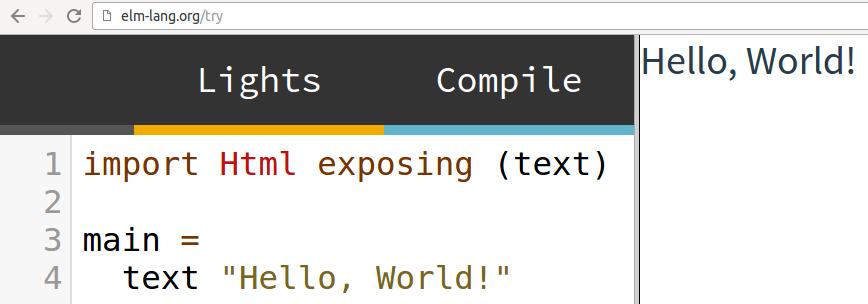
\includegraphics[scale=0.4]{img/elm-try.png}
	\caption{Die Online-\ac{IDE} von Elm}\label{fig:elm-try}
\end{figure}
Die Abbildung~\ref{fig:elm-try} zeigt diese \ac{IDE} mit einem typischen $Hello-World$ Beispiel. Auf der linken Seite ist eigentliche \ac{IDE} erkennbar, während die rechte Seite das Ergebnis nach dem Kompiliervorgang ausgibt. Sollte es einen Fehler während des kompilierens geben, wird die entsprechende Fehlermeldung des $elm-compiler$ dort ausgegeben. Mit Hilfe der Schaltfläche $Lights$ können zum Einen die Farben der \ac{IDE} invertiert werden, während der Knopf $Compile$ den geschriebenen Quellcode kompiliert und ausführt. Kleinere Projekte können entsprechend bequem mit diesem Tool realisiert werden. Die \ac{IDE} bietet einen schnellen Einstieg in die Programmiersprache.


\subsubsection{Installation}
\label{sec:Installation}
Die Online-\ac{IDE} bietet einen schnellen Einstieg in die Programmiersprache, ohne Programme lokal installieren zu müssen. Jedoch sind manche Konzepte nicht in der Online-\ac{IDE} nutzbar, so dass Elm lokal installiert werden muss. Das ist beispielsweise der Fall, sobald spezifische Pakete aus des Paketmanager von Elm installiert und benutzt werden möchten. Mehr Informationen über den Elm-eigenen Paketmanager folgen in der Sektion~\nameref{sec:start-eines-projektes}.

Die Elm-Webseite liefert Anleitungen um Elm auf Windows, Mac und allen NodeJs-kompatiblen Betriebssystemen zu installieren. Im folgenden werden die Kommandos zur Installation von Elm und dem \ac{NPM} unter Ubuntu 14.04 64bit erläutert, da der praktische Teil dieser wissenschaftlichen Arbeit unter diesem Zielsystem vorgenommen wurde.
Die Programmiersprache Elm wird über den \ac{NPM} verbreitet und muss somit zuvor installiert werden. Da der \ac{NPM} wiederum auf der Platform NodeJs basiert, muss auch das dazugehörige Paket installiert werden. Für die Installation sind die Kommandos aus Abbildung~\ref{fig:npm-install} in der Kommandozeile auszuführen.
\begin{figure}[h]
\begin{lstlisting}[language=bash]
$ sudo apt-get update
$ sudo apt-get install nodejs
$ sudo apt-get install npm
\end{lstlisting}
\caption{Installation des \ac{NPM}}\label{fig:npm-install}
\end{figure}
Dadurch wird das NodeJs-Paket installiert und ausführbar gemacht. Anschließend sollte überprüft werden, ob die Installation erfolgreich war und sowohl NodeJS, als auch der \ac{NPM} verfügbar sind.
\begin{figure}[h]
\begin{lstlisting}[language=bash]
$ node -v && npm -v
$ npm install -g elm
\end{lstlisting}
\caption{Installation von Elm}\label{fig:npm-install-check}
\end{figure}
Das Kommando in Zeile $1$ der Abbildung~\ref{fig:npm-install-check} liefert ein Ergebnis, wie es in Abbildung~\ref{fig:npm-installed} zu sehen ist. Elm kann nun über den \ac{NPM} mit dem Kommando aus Zeile $2$ installiert werden. Das Kürzel $-g$ installiert die neueste Elm-Version global für alle Projekte auf dem System. Entfernt man es, wird die Zielversion nur für den aktuellen Ordner zugänglich gemacht. Um die in dieser wissenschaftlichen Arbeit behandelte Version $0.17$ zu installieren, ist der Zusatz $@0.17$ direkt hinter dem globalen Flag notwendig. Nachdem alle Kommandos fehlerfrei ausgeführt wurden sollte Elm über die Konsole nutzbar sein.
\begin{figure}[hb]
\centering
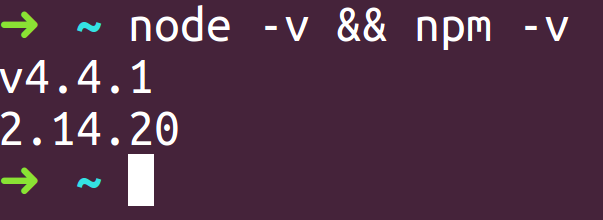
\includegraphics[scale=0.3]{img/npm-nodejs-installation.png}
\caption{Überprüfung der erfolgreichen Installation von NodeJs und dem \ac{NPM}}\label{fig:npm-installed}
\end{figure}


\subsubsection{Start eines Projektes}
\label{sec:start-eines-projektes}
Nachdem die Installation von Elm erfolgreich war, kann nun ein neues Projekt lokal erstellt werden. Dazu gehört zunächst einmal die Initialisierung des Projektordners, wodurch notwendige Ordner erstellt und Pakete installiert werden. Die Entwickler von Elm stellen dafür den Paketmanager $elm-package$ bereit. Dieses Tool wird zur Installation von externen Modulen, sogenannte Bibliotheken oder Pakete, benutzt. Zusätzlich hilft der Paketmanager dabei, das eigene Projekt lauffähig zu halten und nicht durch auftretende Aktualisierungen einzelner Pakete die Lauffähigkeit des eigenen Projektes zu verletzen. Dabei verfolgen die Entwickler des Paketmanagers bestimmte Versionsregeln, die auf jedwede Änderung an einem Paket angewendet wird. Alle Versionsnummern haben dabei genau drei Felder $MAJOR.MINOR.PATCH$, wobei der Beginn der Versionsnummern stets $1.0.0$ ist. Die Felder der Versionsnummern ändern sich abhängig der Änderungen an der API eines Paketes. Die harmloseste Änderung ist dabei der $PATCH$. Das bedeutet, dass die \ac{API} unverändert ist und keinerlei Gefahr für die Lauffähigkeit besteht. Es kann sich hierbei um beispielsweise Verbesserungen eines Algorithmus oder andere interne Änderungen handeln, die jedoch für den außenstehenden Entwickler keine Bedeutung haben.
Der nächstgrößere Schritt stellt die Aktualisierung der $MINOR$ Versionsnummer dar. Wie bei der Aktualisierung auf die nächste $PATCH$-Version, ist auch hier eine Aktualisierung unbedenklich. Das $MINOR$-Feld sagt aus, dass neue Methoden hinzugefügt wurden, alte Methoden jedoch unberührt blieben.
Wichtige Änderungen an einem Paket bei der alte Methoden maßgeblich verändert, oder sogar gelöscht wurden, werden mit dem Feld $MAJOR$ ausgedrückt. Hat sich dieses Feld verändert, wird eine Aktualisierung aller Wahrscheinlichkeit nach dazu führen, dass ein Programm nicht mehr lauffähig ist und Änderungen am eigenen Quellcode vorgenommen werden müssen.
Nutzt ein Entwickler beispielsweise das Paket $elm-lang/html\,1.2.3$, wird es voraussichtlich kompatibel mit allen zukünftigen Versionen bis Version $2.0.0$ sein. Ab diesem Zeitpunkt sind die vorgenommenen Änderungen so massiv, dass eine Aktualisierung nicht ohne weiteres möglich ist. Der Paketmanager $elm-package$ erzwingt die beschriebene Versionierung bei jedem Paket, bevor es veröffentlicht werden kann.TODO: \cite{https://github.com/elm-lang/elm-package}.
\begin{figure}[h]
\centering
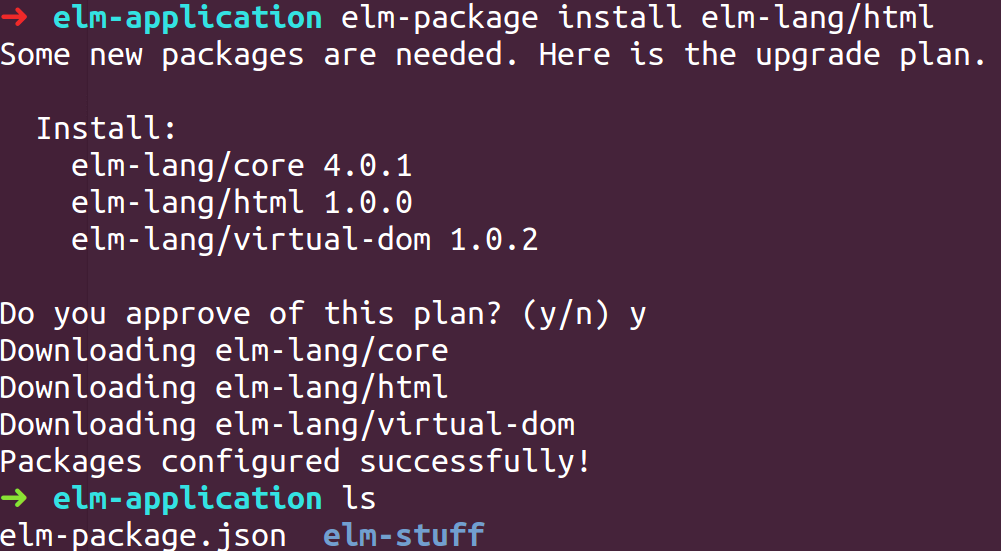
\includegraphics[scale=0.3]{img/elm-setup.png}
\caption{Installation eines externen Paketes über den Elm-Paketmanager}\label{fig:elm-install-package}
\end{figure}
Die Abbildung~\ref{fig:elm-install-package} zeigt, wie ein Paket installiert und der Projektordner eingerichtet wird. Der Paketmanager installiert nach der Bestätigung das angeforderte Paket und alle darin enthaltenen, externen Abhängigkeiten. Des Weiteren wird die Datei $elm-package.json$ erstellt, mit grundlegenden Informationen über das eigene Projekt, wie beispielsweise die Versionsnummer, eine Zusammenfassung oder die zu verwendende Lizenz, sowie eine Liste von installierten externen Paketen. Der Ordner $elm-stuff$ enthält die zuvor installierten Pakete. Nun muss noch manuell eine $.elm$-Datei erstellt werden, üblicherweise mit dem Namen des Projektes. In dieser Datei können die zuvor gezeigten Konzepte genutzt werden, um das gewünschte Programm zu verwirklichen.


\subsubsection{Fertigstellung}
\label{sec:elm-compile}
Zum Kompilieren eines Elm-Programmes wird das Tool $elm-make$ genutzt. Es kompiliert den gesamten Quellcode eines Ordners, oder die Dateien, welche dem Befehl hinzugefügt wurden. Ferne kann der Entwickler entscheiden, ob eine $.html$-Datei erstellt werden soll, in der bereits das kompilierte Elm-Programm eingebaut wird, oder eine $.js$-Datei, so dass das Einbinden oder die Auslieferung selbstständig vorgenommen werden kann.
